The RoboTutor project uses the NAO robot from Aldebaran Technologies as it's embodied agent. The NAO is a humanoid robot with a height of 58 cm. It's size and shape make the NAO suitable for the role of teacher. It is likeable and open, but also makes a serious inpression. Its humanoid looks facilitates social engagement but avoids the uncanny valley effect.\cite{mori1970uncanny}\\

\begin{figure}
\centering
	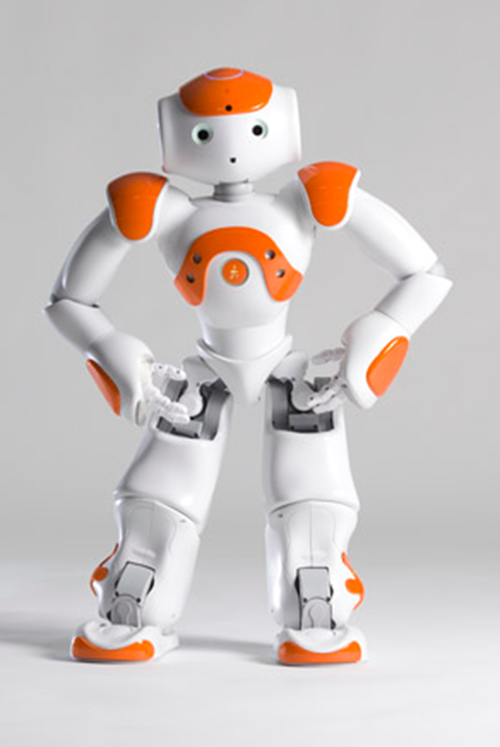
\includegraphics[scale=0.3]{images/NAO.png}
	\caption{The NAO robot}\label{fig:nao}
\end{figure}


The NAO is an out-of-the-box solution that comes with is own hardware. This means no hardware or firmware needs to be developed, allowing for a focus on higher hierarchical layers. This forms a limitation in adaptability, but the NAO provides great flexibility and fills all hardware requirements of the project. \\

The NAO has a flexible body with 25 degrees of freedom that allows it to move naturally and support its communication by body language. It also monitors its 37 sensors that allow it to respond to its audience and surroundings.\\

